\section{Results}
\label{sec:results}

\input{generated/leaderboard\langsuffix}

\subsection{The leaders are not significantly different}
Table~\ref{tab:leaderboard} ranks the \NModels{} models by their overall score. \TopName{} leads with \TopScore{}. In the task-stratified bootstrap (Section~\ref{sec:setup}), the paired difference to the leader is \DiffB{} [\DiffBLo{}, \DiffBHi{}] for \SecondName{}, \DiffC{} [\DiffCLo{}, \DiffCHi{}] for \ThirdName{} and \DiffD{} [\DiffDLo{}, \DiffDHi{}] for \FourthName{}. The three leaders are therefore not significantly different, which does not make them equivalent: \TopName{} comes first in \PTopA{}\,\% of the bootstrap samples, \SecondName{} in \PTopB{}\,\% and \ThirdName{} in \PTopC{}\,\%. Their closeness is partly a ceiling effect, as two of the eight tasks hardly separate API models (Section~\ref{sec:separates}). Below them the API models form a dense band down to \WorstApiName{} (\WorstApiScore{}); the ten local models follow after a gap (Section~\ref{sec:local}).

\subsection{Cost}
\begin{figure}[t]
  \centering
  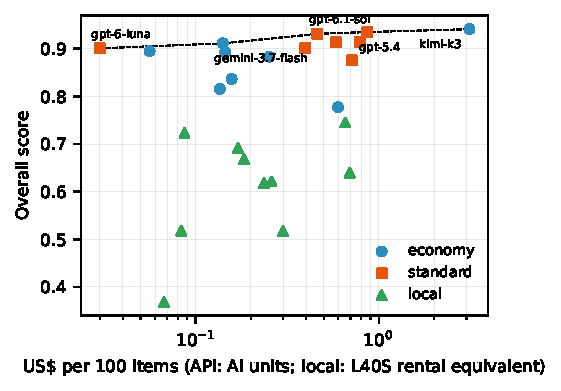
\includegraphics[width=\columnwidth]{pareto}
  \caption{Overall score against cost per 100 items (log scale; API: AI units at US\$0.01; local: GPU time at an on-demand L40S price). The dashed line joins the models that no other model beats at equal or lower cost.}
  \label{fig:pareto}
\end{figure}

The leaders are close in quality but not in price. Per 100 items, \TopName{} costs US\$\TopUSD{}, \SecondName{} US\$\SecondUSD{}, \ThirdName{} US\$\ThirdUSD{} and \FourthName{} US\$\FourthUSD{}. \CheapName{} reaches \CheapScore{}, \CheapGap{} below the leader, for US\$\CheapUSD{}, \CostRatio{} times less than \TopName{}. \ParetoN{} models form the cost--quality front (Fig.~\ref{fig:pareto}): \ParetoNames{}. Price does not follow the tiers we assigned by model names: \TopName{}, grouped with the economy models, is the most expensive per item because it reasons at length (median \TopMedS{}\,s per call against \ThirdMedS{}\,s for \ThirdName{}). The whole study cost US\$\StudyUSD{} in API calls---US\$\AnswerUSD{} for the answers, US\$\JudgeUSD{} for judging them and US\$\ProbeUSD{} for probing the premium models on two items each---and \GpuHours{} GPU-hours for the local models.

\subsection{What separates the models}
\label{sec:separates}
\input{generated/diagnostics\langsuffix}

Not the two knowledge-heavy tasks, which are near ceiling for API models: all \NApi{} answer at least \MethApiMin{} of the methodology questions correctly, and \LangCeil{} of them score at least 0.95 on formal Indonesian (the lowest \LangApiMin{}). This says that these items are too easy for API models, not that the models know the same. The tasks that produce artefacts separate them (Table~\ref{tab:diagnostics}).

\paragraph{References} The widest spread among API models is in the references task (\RefApiMin{}--\RefApiMax{}). Of the references the API models listed, \HalApiMin{}--\HalApiMax{}\,\% are not found in Crossref, and many found ones carry a wrong DOI: the share of listed references with the correct DOI ranges from \DoiApiMin{} to \DoiApiMax{}\,\%. The audit qualifies the misses. Of the \AuditApiNF{} references of API models that Crossref does not know, \AuditApiExact{}\,\% exist with matching title, year and first author in another source---works the Crossref-only score misses---, \AuditApiTitle{}\,\% match only the title of a real work (wrong year or author, or a coinciding generic title), and \AuditApiNone{}\,\% are found nowhere; for the \AuditLocNF{} misses of local models the shares are \AuditLocExact{}, \AuditLocTitle{} and \AuditLocNone{}\,\%. The audit's first pass exposed two Crossref pitfalls that the rule now handles (split subtitles, online-first dates). Per model, \NoneApiMin{}--\NoneApiMax{}\,\% of the references an API model listed are found nowhere (Fig.~\ref{fig:references}). Crediting the works the audit finds as the scorer would raises a references score by at most \VerRefMaxGain{} and leaves the ranking nearly unchanged (Spearman $\rho=\VerRho{}$, largest rank shift \VerMaxShift{}). Models also differ in caution: gpt-5-mini lists \RefsGptFiveMini{} references per item, \NoneGptFiveMini{}\,\% of them found nowhere, gemini-3.7-flash always lists five (\NoneGeminiThreeSevenFlash{}\,\%), and \TopName{} five (\NoneKimiKThree{}\,\%). Because the score counts abstention like an unverifiable reference, cautious models are not rewarded for listing fewer; the share found nowhere is the number to read for safety.

\begin{figure}[t]
  \centering
  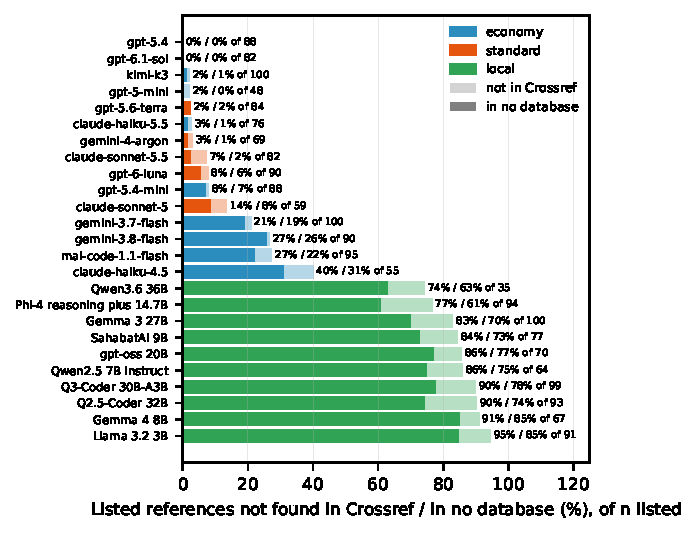
\includegraphics[width=\columnwidth]{references}
  \caption{Share of listed references not found in Crossref (light) and found in none of Crossref, doi.org, Scopus and OpenAlex (dark), with the number of references each model listed for the 20 topics (at most 100).}
  \label{fig:references}
\end{figure}

\paragraph{Outlines} Chapter outlines score \StructApiMin{}--\StructApiMax{} for API models. A frequent mismatch is the test-centred results chapter: \GenericApiMin{}--\GenericApiMax{}\,\% of the API outlines build chapter~IV around assumption, instrument or hypothesis tests for programmes whose theses do not organise their results that way.

\paragraph{Code and LaTeX} \ApiPerfectCode{} of the \NApi{} API models solve every coding task with their first program. Repairing a broken LaTeX document is harder than typesetting a table or a BibTeX entry, which all API models do correctly: the weakest API models produce a compilable document for only \FixApiMin{} of the broken ones.

\paragraph{Grounded writing} By the deterministic checks, API models keep to the given sources: at most \UnsupApiMax{} numbers per review occur in no source, and author--year citations, which the task forbids, appear in at most \ForeignApiMax{}\,\% of their reviews. Several local models ignore the citation format (author--year citations in up to \ForeignLocMax{}\,\% of their reviews).

\subsection{Local models}
\label{sec:local}
\begin{figure}[t]
  \centering
  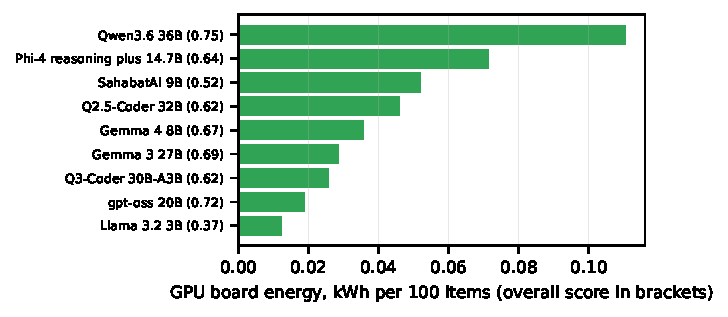
\includegraphics[width=\columnwidth]{energy}
  \caption{GPU board energy per 100 items of the local models (gross; shared server; Qwen2.5 7B not measured), with the overall score in brackets.}
  \label{fig:energy}
\end{figure}

The best local model, \BestLocalName{} (\BestLocalScore{}), stays below the weakest API model, \WorstApiName{} (\WorstApiScore{}). Between the group means the gap is largest for references (\GapRef{}) and code (\GapCode{}), smaller for methodology (\GapMeth{}) and smallest for formal Indonesian (\GapLang{}): local models write formal Indonesian at \LocLangMin{}--\LocLangMax{}, and Qwen3.6 36B scores \TMethodologyQwenThreeSix{} on the methodology questions. Of the references local models list, \NoneLocMin{}--\NoneLocMax{}\,\% are found nowhere, and they solve \LocPassOneMin{}--\LocPassOneMax{} of the coding tasks with their first program (mean \LocPassOneMean{}, rising to \LocRepairMean{} after one repair turn). The Indonesian-tuned SahabatAI 9B scores lower on formal Indonesian than the general Gemma~4 8B (\SahLang{} against \GemmaFourLang{}) and fails at code (\SahCode{}), so its overall score (\SahOverall{}) stays below Gemma~4's (\GemmaFourOverall{}). At an on-demand L40S price and three parallel requests, local models cost US\$\LocUSDMin{}--\LocUSDMax{} per 100 items, no less than the cheapest API models, and drew \LocKwhMin{}--\LocKwhMax{}\,kWh per 100 items (Fig.~\ref{fig:energy}); gpt-oss 20B gives the most score per kWh in this setup (\ScoreGptOss{} for \KwhGptOss{}\,kWh and US\$\UsdGptOss{} per 100 items).

\subsection{Judges and provenance}
The three judges rated \NJudgedAnswers{} answers with \NJudgeCalls{} ratings. On the \NAllJudges{} answers that all three rated (candidates from vendors other than the judges'), their mean ratings agree with Krippendorff's $\alpha=\AlphaJudges{}$ (interval); single criteria agree less ($\alpha$ from \AlphaCritMin{} to \AlphaCritMax{}, ordinal), least for instruction compliance and faithfulness. The judges' leniency differs by up to \LeniencyRange{} on the 0--1 scale, which the calibration removes. Their scores follow the deterministic checks: Spearman's $\rho$ is \RhoAnsGrd{} (grounded) and \RhoAnsLng{} (language) across answers, and \RhoModelGrd{} and \RhoModelLng{} across model means. The extraction panel agreed unanimously on \SilverUnanimous{}\,\% of the fields; analysis techniques were the hardest field (no majority on \SilverAnalysisNone{} of 30 excerpts, which are therefore not scored). In all \NApiCalls{} API calls of the study the SDK reported the requested model as the one that answered: the silent substitution reported for the same SDK when an account is not entitled to a model~\cite{arya2026paperagent} did not occur here. The check rests on the SDK's own usage event, not on an independent test of the backend.
